We present the integration of Jupyter Notebooks into the MathHub system.

\ednote{TW: Update this with the actual MH Structure}

\subsection{Overview}

\begin{newpart}{FR@TW: check if true}
Our system consists of four components:
\begin{compactitem}
\item A GitLab repository hosting server\footnote{\url{http://gl.mathhub.info}} provides persistent storage of documents in any format, including their OMDoc representation.
\item An MMT instance\footnote{\url{http://mmt.mathhub.info}} uses the OMDoc representations to provides the shared knowledge space and provides a high-level API for it.
\item A Jupyter Notebook server\footnote{\url{http://jupyter.mathhub.info}} provides web-based IDE for editing interactive documents.
\item The MathHub frontend\footnote{\url{http://mathhub.info}} serves as the main entry point and delegates some subtasks to the former.
\end{compactitem}

The Jupyter server is an out of the box installation of Jupyter except for additionally supporting our new MMT kernel.
\ednote{Update URL strucure}
Consequently, the integration between the Jupyter and the MathHub frontends is shallow: MathHub opens Jupyter Notebooks in separate tabs or iframes using URLs served by Jupyter.
We would have preferred to deeply integrate the Jupyter frontend into MathHub, e.g., by using Jupyter simply as a JavaScript library in MathHub.
But that is infeasible because Jupyter is primarily used as a monolithic system not designed to allow deep integration.\footnote{The most recent versions of Jupyter are aiming to allow it, but at present any deep integration would realistically be too brittle to be worthwhile.}
\end{newpart}

\subsection{Notebooks as Standalone Documents}

The MathHub frontend already provides special interaction functionality for individual document types.
We used this by making Jupyter Notebooks a new document type; see Figure~\ref{fig:mathhub-NB} for an example.
When displaying a known document type, the frontend shows multiple tabs.
For Notebooks, these are the following:
\begin{compactenum}[\em i\rm)]
\item \textsf{view} gives a preview of the notebook, essentially the computation cells without output, pre-rendered for static serving without involving Jupyter at all.%
\ednote{MK: we should implement this; I am not sure what the best way is for this. I guess a build target based on \texttt{https://github.com/jendas1/jupyter-notebook-quick-look}.}
\item \textsf{run/edit} opens the respective notebook on the Jupyter server for execution and editing.
Any changes to the Notebook made from within Jupyter can be committed back to the Git repository. 
\item \textsf{metadata} (this is the tab open in Figure~\ref{fig:mathhub-NB}), shows the metadata provided by the Jupyter kernel and the repository. 
\item \textsf{source} provides access to the document source; here simply a link to the notebook file in the Git repository.
\item \textsf{statistics} shows statistical information about the notebook, its corresponding MMT document, and its connections with other MMT documents in the background knowledge base.
\item \textsf{graph} links to graph-based visualizations of the document including the theory graph, declaration graph, and dependency graph, using our TGView system, a canvas-based in-browser visualizer for knowledge graph information~\cite{RupKohMue:fitgv17}.
\end{compactenum}
This integration combines the interactive features of the Jupyter server with the knowledge management facilities on MathHub. In the future, we plan to integrate the notebook diff/patch \textsf{nbdime} developed in OpenDreamKit to extend the knowledge management facilities. 

\begin{figure}[ht]\centering
  \fbox{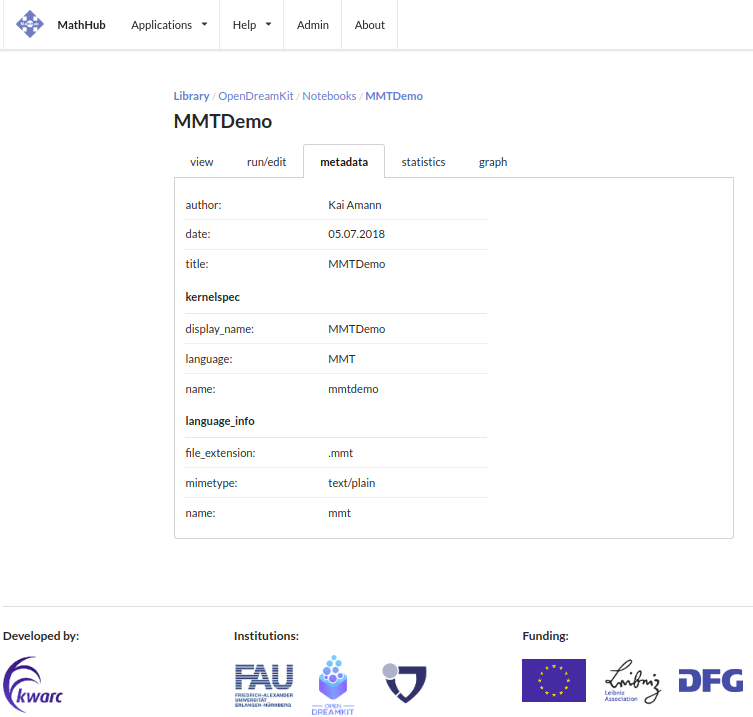
\includegraphics[width=13cm]{../D4.11/NB-Mathhub}}
  \caption{A Jupyter Notebook in MathHub (Metadata)}\label{fig:mathhub-NB}
\end{figure}
\ednote{TW: Wait, this exists?}
%A Jupyter Notebook additionally has a special button appears that allows users to open the notebook in the associated Jupyter server. Currently these notebooks do not use the MMT process running on MathHub.info, due to the architecture of the MMT Kernel. Therefore they currently do not have access to the MathHub universe. \ednote{KA: if the Kernel server would run on the same VM as the MathHub MMT we could give the kernel access to it}
%\ednote{@Kai, @Tom: check this, do the implementation}

\ednote{@KA: write the example from Fig.~\ref{fig:test_theory} as a Jupyter notebook, store the file somewhere on gl.mathhub.info and give a link to the Fig.~\ref{fig:mathhub-NB} view of that notebook}

\subsection{Notebooks as Parts of Static Documents}

To interact dynamically with content in arbitrary MathHub documents, we added a new feature that creates a new ephemeral Jupyter Notebook and inserts it (via an iframe) into the current document.
Importantly, the new Notebook is prefilled with an import of the current context so that users can Here we can feed the document context information into the interior notebook.

\begin{figure}[ht]\centering
  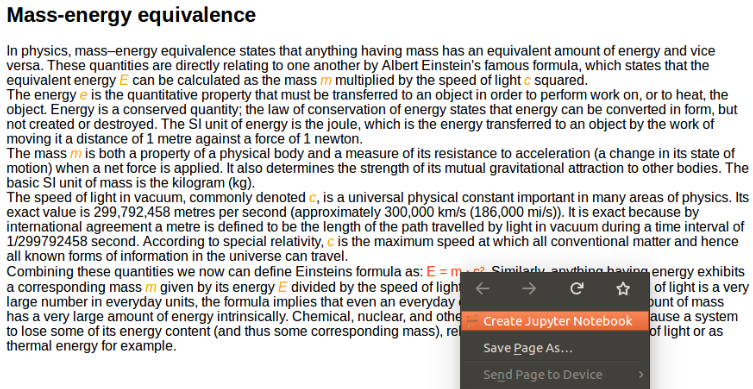
\includegraphics[width=15cm]{../D4.11/conversionHTML}
  \caption{HTML document and the context menu for converting}\label{fig:conversionHTML}
\end{figure}
\ednote{Re-do this screenshot cleanly}

Continuing the example from the previous section, Figure~\ref{fig:conversionHTML} shows a scientific HTML document that contains the equation $E=mc^2$.
\ednote{MK@KA/FR: We should make an sTeX document that contains $E=mc^2$ (e.g. by copying parts of \texttt{https://en.wikipedia.org/wiki/Mass-energy\_equivalence}) and really implement the in-document computation example.}
The user can use the context menu to trigger the notebook generation on this formula.
The context menu is generated using JavaScript that picks up on annotations of formulas with specific CSS classes.
Currently the author has to manually annotate the formulas, but we are working on a mechanism to automatically create it from the document context.

\ednote{Describe structure of tags within the HTML}
Figure~\ref{fig:conversionNotebook} shows the notebook created by our tool.
Note that the generated notebook starts with several \texttt{include} declarations that import the context of the formula.
These are generated by MathHub to obtain a minimal standalone MMT theory in which the respective formula is well-formed. 

If desired, the notebooks can be easily uploaded to the Jupyter server, stored persistently in the repository server, or evaluated in a locally deployed version of the system per drag-and-drop.

%The two predominant cell types in Jupyter notebooks are \texttt{code} and \texttt{markdown} cells. 
%Code Cells contain user input, like described in section \ref{sec:kernel:syntax}.
%The HTML elements that contain the input for these code cells are usually not visible, since they do not fit into the context of a scientific document and may not be understood by reviewers that are not familiar with MMT syntax. 
%The other cell type: markdown cells, can contain any type of plain text and support GitHub flavoured markdown. 
%Therefore markdown cells are used for providing notebooks with additional selectable information from the original HTML document.

\begin{figure}[ht]\centering
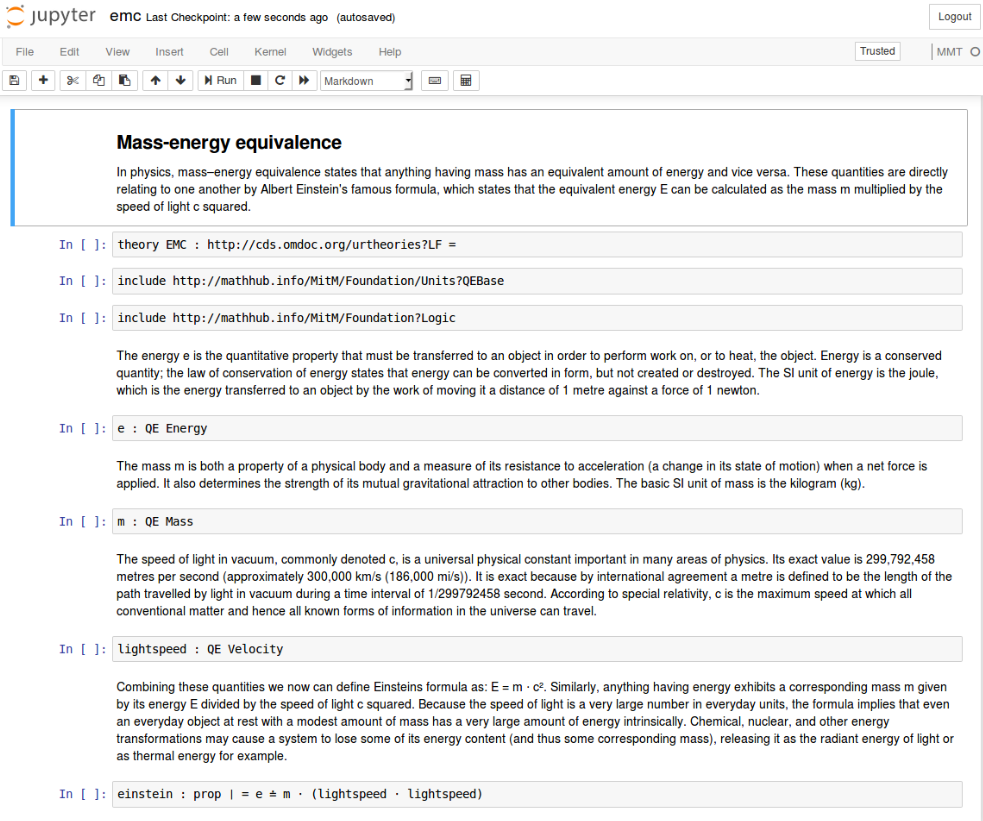
\includegraphics[width=15cm]{../D4.11/conversionNotebook}
\caption{The resulting Jupyter notebook}
\label{fig:conversionNotebook}
\end{figure}
\ednote{run all cells}

%%% Local Variables:
%%% mode: latex
%%% mode: visual-line
%%% fill-column: 5000
%%% TeX-master: "paper"
%%% End:

%  LocalWords:  Jupyter ednote compactenum textsf texttt visualizations RupKohMue:fitgv17 nbdime centering fbox includegraphics NB-Mathhub
